\documentclass[a4paper,12pt]{article}

% Paquetes necesarios
\usepackage[utf8]{inputenc}   % Codificación de caracteres
\usepackage[spanish]{babel}   % Idioma español
\usepackage{amsmath, amssymb} % Símbolos matemáticos
\usepackage{graphicx}         % Inclusión de gráficos
\usepackage{cite}             % Gestión de citas
\usepackage{hyperref}         % Enlaces y referencias
\usepackage{geometry}         % Configuración de márgenes
\usepackage{fancyhdr}         % Encabezados y pies de página
\usepackage{titlesec}         % Formato de títulos
\usepackage{booktabs}         % Tablas profesionales
\usepackage{caption}          % Personalización de leyendas
\usepackage{enumitem}         % Personalización de listas
\include{float}

% Configuración de márgenes
\geometry{left=3cm, right=3cm, top=2.5cm, bottom=2.5cm}

% Configuración de encabezados y pies de página
\setlength{\headheight}{14.49998pt}
\pagestyle{fancy}
\fancyhf{}
\fancyhead[L]{Univesidad de Granada}
%\fancyhead[C]{Escuela Técnica Superior de Ingeniería Informática}
\fancyhead[R]{ISE: Prácticas del Bloque 1}
\fancyfoot[L]{Ismael Sallami Moreno}
\fancyfoot[C]{\thepage}
\fancyfoot[R]{\today}

% Formato de títulos
\titleformat{\section}{\large\bfseries}{\thesection.}{0.5em}{}
\titleformat{\subsection}{\normalsize\bfseries}{\thesubsection.}{0.5em}{}

% Datos del documento
\title{\textbf{Práctica 1 de Ingeniería de Servidores}}
\author{
    Ismael Sallami Moreno \\
    \texttt{ism350zsallami@correo.ugr.es}
}
\date{
    \vspace{1cm}
    \begin{tabular}{rl}
        \textbf{Asignatura:} & Ingeniería de Servidores \\
        \textbf{Tema:} & VirtualBox con Rocky \\
        \textbf{Fecha:} & \today
    \end{tabular}
}

\begin{document}

% Portada
\maketitle
\begin{center}
    
\includegraphics[width=0.5\textwidth]{images/logo_ugr.png}
\end{center}
\newpage

% Resumen
\begin{abstract}
\noindent
\textbf{Resumen:} Este documento presenta una plantilla en LaTeX para la elaboración de trabajos académicos en el ámbito tecnológico. Se incluyen secciones típicas como introducción, metodología, resultados y conclusiones, así como el formato para las referencias bibliográficas.
\end{abstract}
\bigskip


% Tabla de contenidos
\tableofcontents
\newpage

\section{Ejercicio 1 Opcional}
El alumno/a debe ser capaz de presentar un MV con la configuración descrita en este apartado. La configuración debe ser permanente, es decir, en todo caso, tras reiniciar el equipo, la configuración será la esperada.
Para validar la configuración de red, el alumno/a debe ser capaz de:
\begin{itemize}
    \item Hacer ping desde el equipo anfitrión a la MV y viceversa.
    \item Hacer ping desde la MV a cualquier equipo accesible públicamente en Internet por FQHN o IP.
    \item Conectar por ssh desde el equipo anfitrión a la MV .
\end{itemize}

\subsection{Solución}
Una vez que hayamos instalado el SO que se nos pide correctamente. Debemos de realizar una serie de ajustes previos:
\begin{itemize}
    \item Añadir nuestro usuario, para ello debemos de ejecutar lo siguientes comandos (iniciando como usuario root):
    \begin{itemize}
        \item \texttt{sudo useradd nombre\_de\_usuario}        
        \item \texttt{sudo passwd nombre\_de\_usuario}
        \item \texttt{sudo usermod -aG wheel nombre\_de\_usuario} para que pueda usar el comando sudo.
    \end{itemize}
\end{itemize}

\begin{itemize}
    \item Configurar la red NAT y una de tipo Host-Only, para ello en Herramientas en la VM debemos seleccionar la opción de Red y añadir una nueva interfaz de red de tipo Host-Only, y paso seguido configurar la red NAT (ver Figura 1 y 2 )
    \item Comprobar que el servicio SSH está instalado, por defecto se suele instalar, para asegurarnos debemos de ejecutar el comando \texttt{sudo systemctl status ssh}. En el caso de que no venga instalado debemos de ejecutar el comando \texttt{sudo dnf install -y openssh-server openssh-clients}\footnote{Incluimos clients para añadir el servicio de cliente.} (Ver Figura 5).
    \item Cambiar la variable PS1 como se nos pedía, para ello debemos de editar el fichero de bashrc y exportar la variable PS1 con el valor que se nos pedía:
    \begin{itemize}
        \item \texttt{PS1='\textbackslash u@\textbackslash h:\textbackslash t:\textbackslash w\textbackslash\$ '} (Ver Figura 5), donde:
        \begin{itemize}
            \item \texttt{\textbackslash u}: Nombre del usuario actual.
            \item \texttt{\textbackslash h}: Nombre del hostname (nombre del sistema).
            \item \texttt{\textbackslash t}: Hora actual en formato de 24 horas (HH:MM:SS).
            \item \texttt{\textbackslash w}: Directorio de trabajo actual.
            \item \texttt{\$}: Símbolo del prompt, que será \$ para un usuario normal y \# para root.
        \end{itemize}
    \end{itemize}
\end{itemize}

\begin{figure}[htbp]
    \centering
    \begin{minipage}[b]{0.45\textwidth}
        \centering
        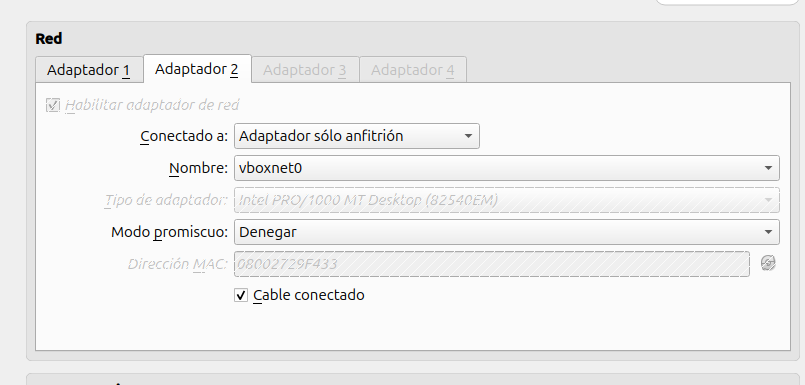
\includegraphics[width=\textwidth]{images/adaptador2.png}
        \caption{Configuración de la red NAT y Host-Only}
        \label{fig:ejercicio1}
    \end{minipage}
    \hfill
    \begin{minipage}[b]{0.45\textwidth}
        \centering
        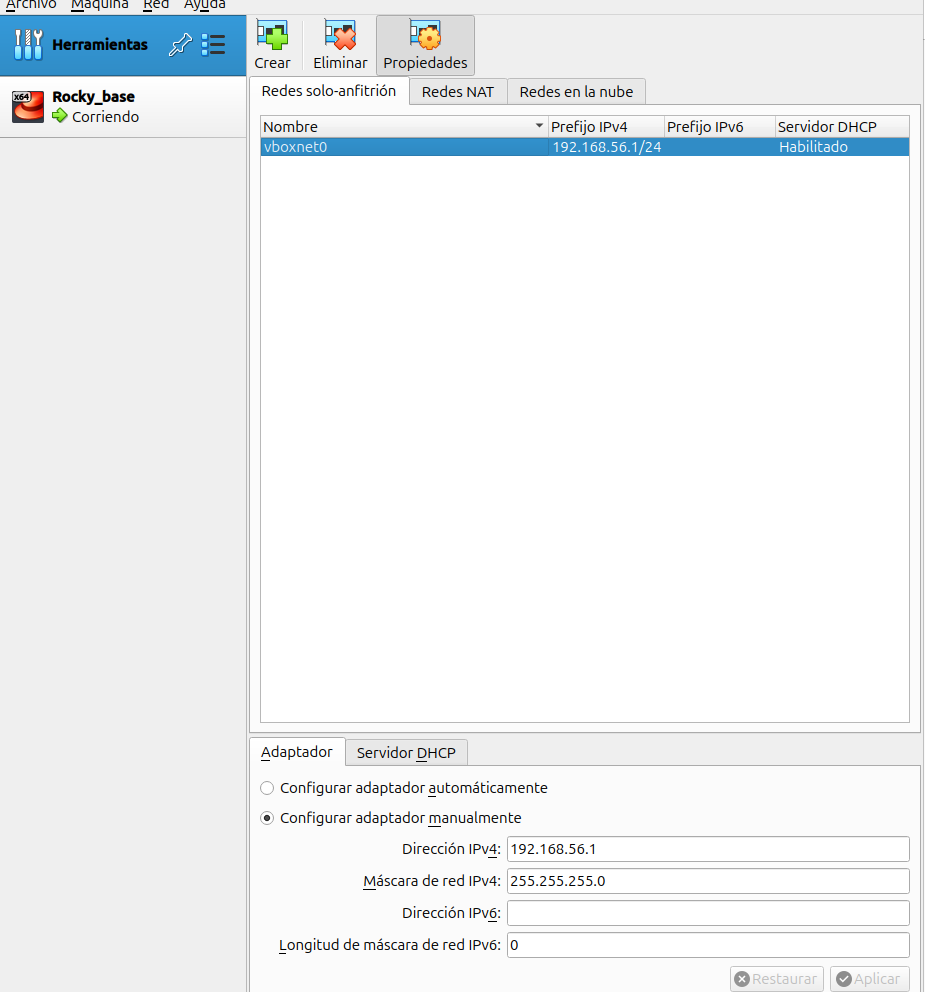
\includegraphics[width=\textwidth]{images/vbox.png}
        \caption{Configuración de VirtualBox para la red de Host-Only}
        \label{fig:ejercicio1_vbox}
    \end{minipage}
\end{figure}

Además se nos pide que la Ip de Host Only sea estática, para ello vamos a asegurarnos usando la herramienta \textit{nmtui}, en la que vamos a ver si es estática o no la ip. Como podemos ver en la siguiente imagen esta configurada como ip automática, que viene siendo lo mismo que dinámica por lo que debemos de cambiarlo a manual para poder configurar la ip estática. (Ver Figura 3 y 4). Para ver que efectivamente la ip cambió, podemos verlo en la Figura 5.
\begin{figure}[htbp]
    \centering
    \begin{minipage}[b]{0.45\textwidth}
        \centering
        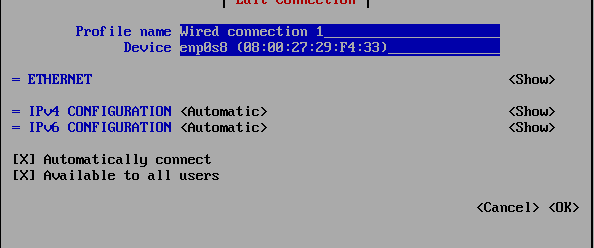
\includegraphics[width=\textwidth]{images/nmtui1.png}
        \caption{Con nmtui vemos que es dinámica}
        \label{fig:ejercicio1}
    \end{minipage}
    \hfill
    \begin{minipage}[b]{0.45\textwidth}
        \centering
        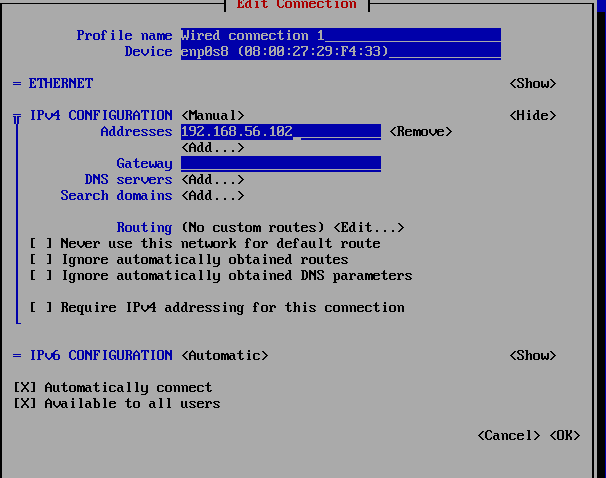
\includegraphics[width=\textwidth]{images/nmtui_2.png}
        \caption{Cambiamos a manual y asignamos una ip estática válida}
        \label{fig:ejercicio1_vbox}
    \end{minipage}
\end{figure}



\begin{figure}
    \centering
    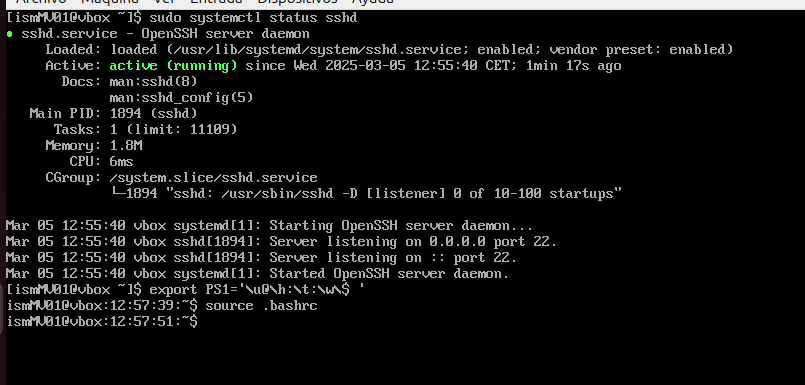
\includegraphics[width=0.8\textwidth]{images/sshd_PS1.png}
    \caption{Sshd y variable PS1}
    \label{fig:ejercicio1_1}
\end{figure}

\begin{figure}
    \centering
    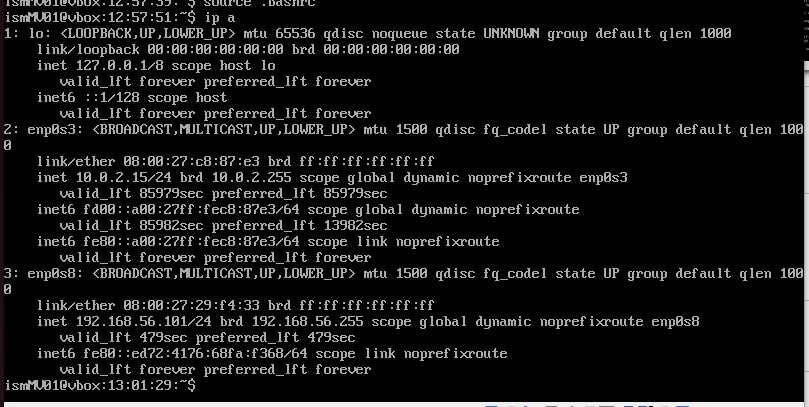
\includegraphics[width=0.8\textwidth]{images/resultado_ipa.png}
    \caption{Resultado de ip a}
    \label{fig:ejercicio1_2}
\end{figure}

Una vez hayamos cambiado la ip estática, debemos de verificar que efectivamente se ha cambiado y para ello usamos el comando \texttt{ip a} y vemos que efectivamente se ha cambiado la ip a la que hemos asignado. (Ver Figura 7).

\begin{figure}
    \centering
    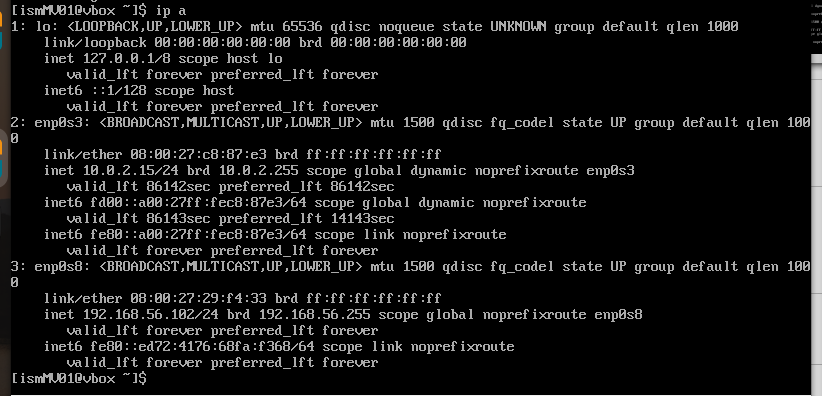
\includegraphics[width=0.8\textwidth]{images/ping2.png}
    \caption{Resultado de ip a para verificar el cambio de ip}
    \label{fig:ejercicio1_2}
\end{figure}

Llegado a este punto vamos a realizar un ping a la máquina anfitriona y viceversa, para ello usamos el comando \texttt{ping -c <número de pings> ip\_de\_la\_maquina} y vemos que efectivamente hay conexión entre ambas máquinas. (Ver Figura 8, 9 y 10). Además, vemos que gracias al \textit{NAT} podemos hacer ping a cualquier máquina accesible en internet\footnote{Cabe destacar que durante el desarrollo de la actividad, surgían algunas problemas con NetworkManager, polkiy y DBus, pero se solucionaban al reiniciarlos o bien reinstalarlos}. (Ver Figura 11).

\begin{figure}[htbp]
    \centering
    \begin{minipage}[b]{0.45\textwidth}
        \centering
        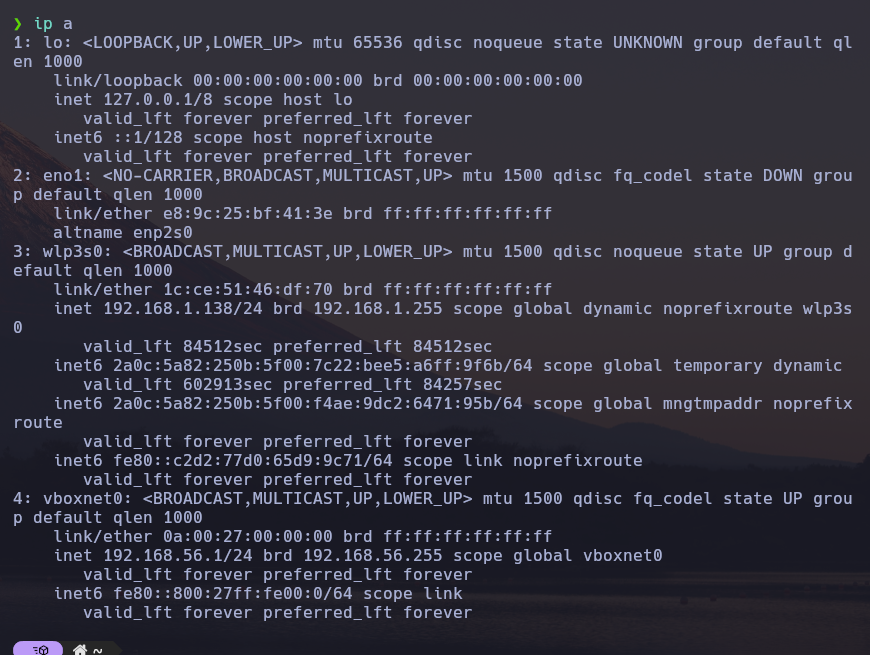
\includegraphics[width=\textwidth]{images/ip_a_host.png}
        \caption{Resultado del comando de \textit{ip a } en la máquina anfitriona para ver la ip}
        \label{fig:ejercicio1}
    \end{minipage}
    \hfill
    \begin{minipage}[b]{0.45\textwidth}
        \centering
        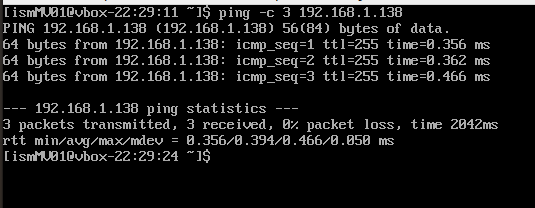
\includegraphics[width=\textwidth]{images/ping_a_anfitriona.png}
        \caption{Ping a la máquina anfitriona}
        \label{fig:ejercicio1_vbox}
    \end{minipage}
\end{figure}


\begin{figure}[htbp]
    \centering
    \begin{minipage}[b]{0.45\textwidth}
        \centering
        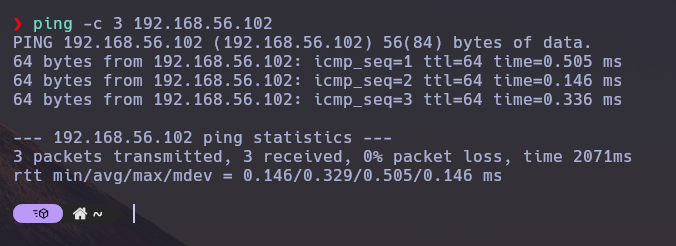
\includegraphics[width=\textwidth]{images/ping_anf_a_mv.png}
        \caption{Ping de la máquina anfitriona a la máquina virtual}
        \label{fig:ejercicio1}
    \end{minipage}
    \hfill
    \begin{minipage}[b]{0.45\textwidth}
        \centering
        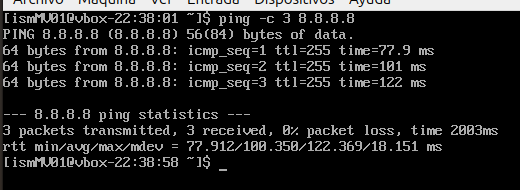
\includegraphics[width=\textwidth]{images/ping_fuera.png}
        \caption{Ping a un servidor público (Google)}
        \label{fig:ejercicio1_vbox}
    \end{minipage}
\end{figure}


En cuanto al servicio ssh, debemos de ver el estado del servicio sshd con el comando \texttt{sudo systemctl status sshd} y vemos que esta corriendo. En este punto desde el anfitrión podemos introducirt la línea de comando \texttt{ssh ismMV01@192.168.56.102} y vemos que efectivamente todo funciona correctamente. (Ver Figura 12 y 13).






\begin{figure}[htbp]
    \centering
    \begin{minipage}[b]{0.45\textwidth}
        \centering
        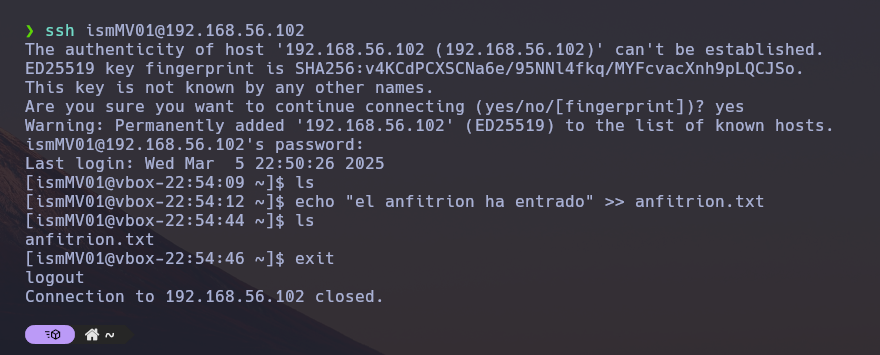
\includegraphics[width=\textwidth]{images/ssh1.png}
        \caption{Ssh en la máquina anfitriona y creación de un archivo en la MV}
        \label{fig:ejercicio1}
    \end{minipage}
    \hfill
    \begin{minipage}[b]{0.45\textwidth}
        \centering
        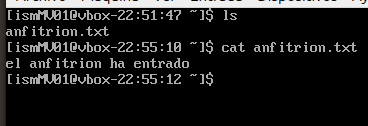
\includegraphics[width=\textwidth]{images/ssh2.png}
        \caption{Ver el contenido del archivo creado en la MV desde el anfitrión}
        \label{fig:ejercicio1_vbox}
    \end{minipage}
\end{figure}









\newpage
% Referencias
\begin{thebibliography}{99}
\bibitem{Referencia1}
Autor(es), \emph{Título del artículo}, Nombre de la Revista, volumen(número), páginas, año.

\bibitem{Referencia2}
Autor(es), \emph{Título del libro}, Editorial, año.

\bibitem{Referencia3}
Autor(es), \emph{Título del documento}, Nombre de la Conferencia, páginas, año.
\end{thebibliography}

\end{document}